\documentclass[aspectratio=169,12pt]{beamer}

% ============================================================
% PACOTES
% ============================================================
\usepackage[utf8]{inputenc}
\usepackage[T1]{fontenc}
\usepackage[brazil]{babel}
\usepackage{amsmath,amssymb,amsfonts}
\usepackage{graphicx}
\usepackage{booktabs}
\usepackage{multirow}
\usepackage{array}
\usepackage{colortbl}
\usepackage{xcolor}
\usepackage{tikz}
\usepackage{adjustbox}
\usepackage{appendixnumberbeamer}

% ============================================================
% TEMA E CORES
% ============================================================
\usetheme{Madrid}
\usecolortheme{whale}
\setbeamertemplate{navigation symbols}{}
\setbeamertemplate{footline}[frame number]
\setbeamerfont{footnote}{size=\tiny}

\definecolor{darkblue}{RGB}{0,51,102}
\definecolor{lightblue}{RGB}{51,122,183}
\definecolor{darkgreen}{RGB}{0,128,0}
\definecolor{darkred}{RGB}{178,34,34}
\definecolor{lightyellow}{RGB}{255,255,224}
\definecolor{lightgray}{RGB}{245,245,245}

\setbeamercolor{title}{fg=white,bg=darkblue}
\setbeamercolor{frametitle}{fg=white,bg=darkblue}
\setbeamercolor{block title}{bg=lightblue,fg=white}
\setbeamercolor{block body}{bg=lightgray}

\newcommand{\highlight}[1]{\textcolor{darkblue}{\textbf{#1}}}
\newcommand{\warn}[1]{\textcolor{darkred}{\textbf{#1}}}
\newcommand{\good}[1]{\textcolor{darkgreen}{\textbf{#1}}}

% ============================================================
% INFORMACOES
% ============================================================
\title[Decisões de LLMs via Otimização Inversa]{Explicando Decisões de LLMs\\via Otimização Inversa}
\author{George Gomes}
\institute{Programa de Pós-Graduação}
\date{2026}

% ============================================================
\begin{document}

% ============================================================
% SLIDE 1: TITULO
% ============================================================
\begin{frame}[plain]
\titlepage
\end{frame}

% ============================================================
% PARTE 1 — INTRODUCAO E MOTIVACAO
% ============================================================

% ============================================================
% SLIDE 2: MOTIVACAO
% ============================================================
\begin{frame}{Motivação --- Por que investigar decisões de LLMs?}
\begin{itemize}
    \item LLMs são \highlight{``caixas-pretas''}: tomam decisões mas não explicam o critério
    \item \textbf{Pergunta central:}
    \begin{quote}
        \emph{``LLMs possuem um processo de decisão \highlight{estável} e \highlight{aprendível}?''}
    \end{quote}
    \item Se sim $\Rightarrow$ podemos extrair uma \highlight{métrica matemática} ($\hat{W}$) que \textbf{explique} e \textbf{preveja} suas decisões
    \item \textbf{Relevância:}
    \begin{itemize}
        \item Explainability / Interpretabilidade
        \item Confiança em sistemas de IA
        \item Auditoria de decisões automatizadas
    \end{itemize}
\end{itemize}
\end{frame}

% ============================================================
% SLIDE 3: HIPOTESES
% ============================================================
\begin{frame}{Hipóteses do Trabalho}
\begin{description}
    \item[\textbf{H1}] \textbf{Consistência:} O LLM mantém o mesmo critério decisório em problemas diferentes
    \item[\textbf{H2}] \textbf{Few-shot amplifica:} Exemplos rotulados aumentam a concordância LLM--métrica
    \item[\textbf{H3}] \textbf{LLM como aprendiz:} O LLM consegue aprender o critério de um perito externo
    \item[\textbf{H4}] \textbf{Exemplos difíceis:} Exemplos próximos à fronteira são mais informativos
    \item[\textbf{H5}] \textbf{Estabilidade:} O comportamento é reproduzível entre execuções
\end{description}
\end{frame}

% ============================================================
% SLIDE 4: ABORDAGEM
% ============================================================
\begin{frame}{Abordagem --- Otimização Inversa}
\begin{block}{Ideia Geral}
A partir das \textbf{decisões observadas} do LLM, aprender a \textbf{função objetivo implícita}.
\end{block}

\vspace{0.3cm}
\textbf{Métrica de Mahalanobis diagonal:}
\[
d_W(\mathbf{x}, \mathbf{c}) = \sqrt{\sum_{i} w_i \cdot (x_i - c_i)^2}, \quad w_i \geq 0
\]

\textbf{Por que diagonal?}
\begin{itemize}
    \item Simplicidade: $O(d)$ parâmetros vs.\ $O(d^2)$ na Mahalanobis completa
    \item Interpretabilidade: cada $w_i$ indica a importância da feature $i$
    \item Tratabilidade computacional
\end{itemize}

\textbf{Classificação:} nearest-centroid --- atribuir ao centróide mais próximo sob $W$.
\end{frame}


% ============================================================
% PARTE 2 — DESIGN EXPERIMENTAL
% ============================================================

% ============================================================
% SLIDE 5: VISAO GERAL DOS DADOS
% ============================================================
\begin{frame}{Dados Sintéticos 2D --- Visão Geral}
\begin{columns}
\column{0.55\textwidth}
\begin{itemize}
    \item 4 problemas gerados com \texttt{make\_blobs}
    \item Distribuições Gaussianas bidimensionais
    \item Dados 2D permitem \textbf{visualização direta} das fronteiras de decisão
    \item Cada problema tem geometria distinta
\end{itemize}
\column{0.45\textwidth}
\begin{center}
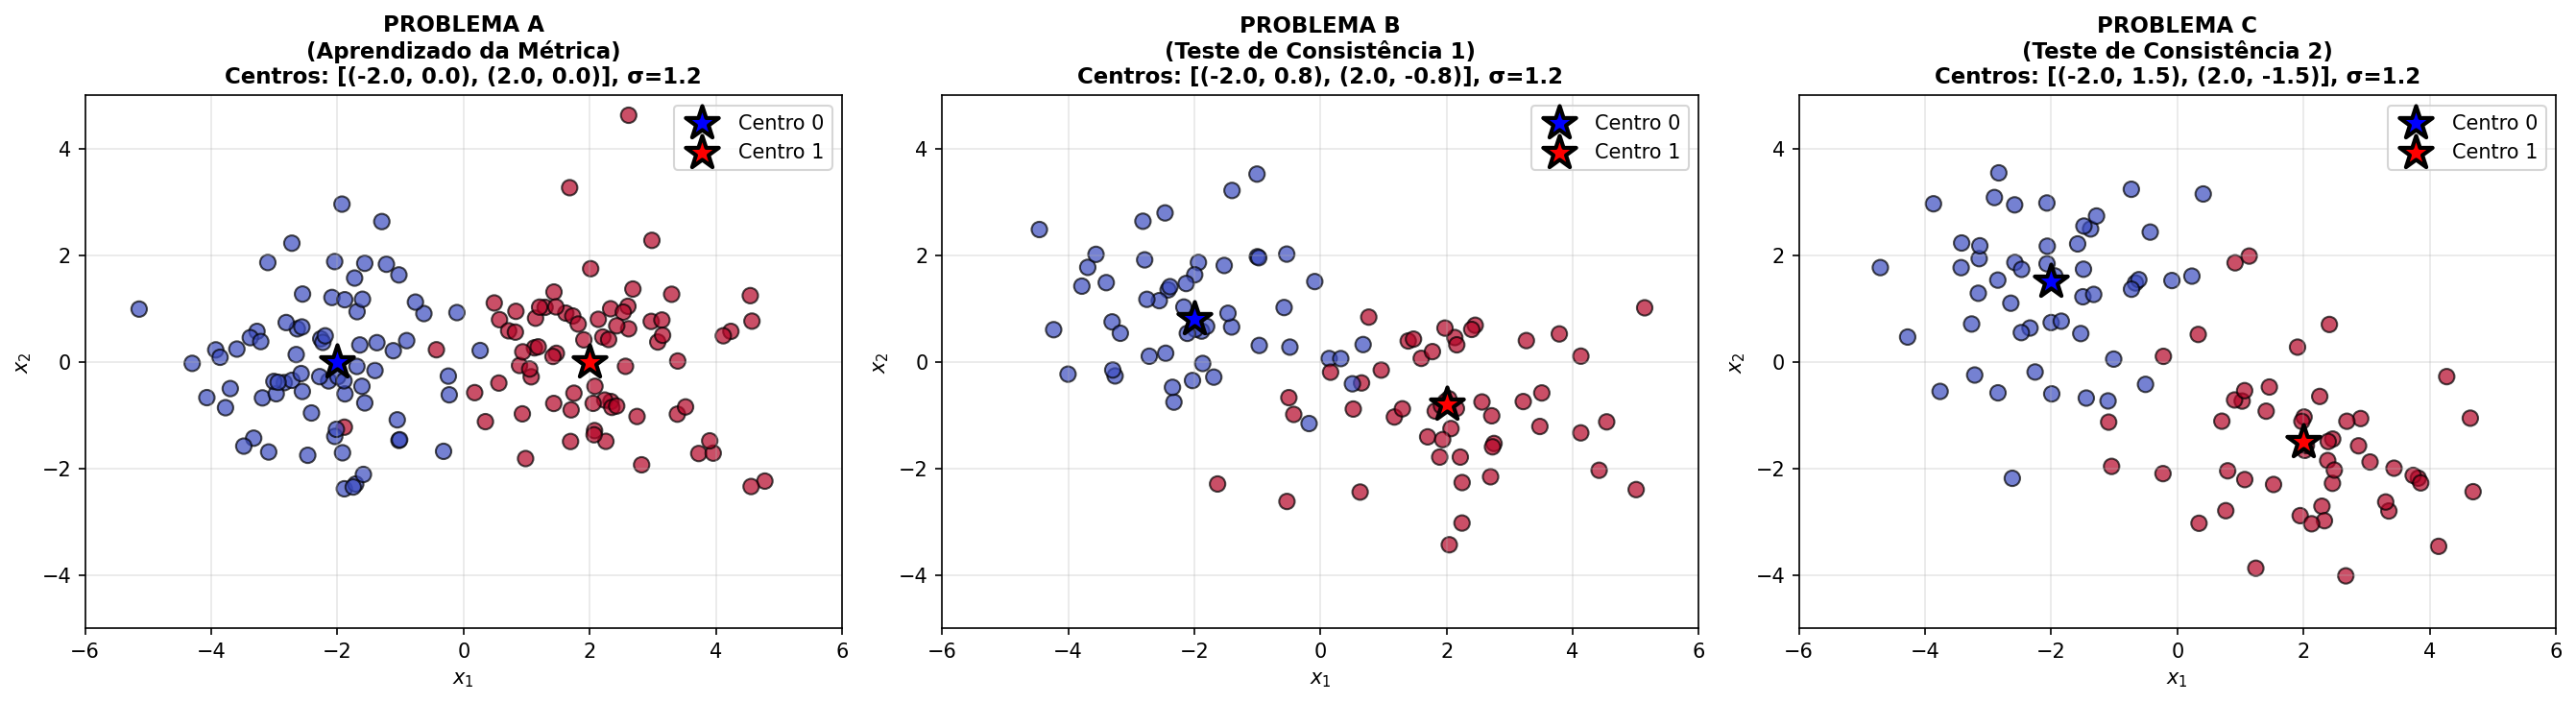
\includegraphics[width=\textwidth]{../01_all_three_problems.png}
\end{center}
\end{columns}
\end{frame}

% ============================================================
% SLIDE 6: PROBLEMA A
% ============================================================
\begin{frame}{Problema A --- Treino da Métrica}
\begin{columns}
\column{0.5\textwidth}
\begin{itemize}
    \item \textbf{150 pontos}, 2 classes
    \item Usado na \textbf{Fase A}: LLM classifica em zero-shot
    \item A partir das decisões, aprende-se $\hat{W}_{\text{LLM}}$
    \item Parâmetros: centroides e \texttt{cluster\_std} do \texttt{make\_blobs}
\end{itemize}
\column{0.5\textwidth}
\begin{center}

\includegraphics[width=\textwidth]{../16_dataset_overview_seed42.png}
\end{center}
\end{columns}
\end{frame}

% ============================================================
% SLIDE 7: PROBLEMA B
% ============================================================
\begin{frame}{Problema B --- Teste de Consistência 1}
\begin{columns}
\column{0.55\textwidth}
\begin{itemize}
    \item \textbf{100 pontos}, centroides deslocados verticalmente
    \item Geometria \textbf{diferente} do Problema A
    \item Testa se $\hat{W}_{\text{LLM}}$ aprendida na Fase A \textbf{generaliza}
    \item Mesmo número de classes, distribuição distinta
\end{itemize}
\column{0.45\textwidth}
\begin{center}

\includegraphics[width=0.95\textwidth]{../16_dataset_overview_seed42.png}
\end{center}
\end{columns}
\end{frame}

% ============================================================
% SLIDE 8: PROBLEMA C
% ============================================================
\begin{frame}{Problema C --- Teste de Consistência 2}
\begin{columns}
\column{0.55\textwidth}
\begin{itemize}
    \item \textbf{100 pontos}, distorção geométrica maior
    \item Teste mais \textbf{desafiador} que o Problema B
    \item Validação adicional da generalização da métrica
    \item Se a consistência se mantém $\Rightarrow$ evidência forte de estabilidade
\end{itemize}
\column{0.45\textwidth}
\begin{center}

\includegraphics[width=0.95\textwidth]{../16_dataset_overview_seed42.png}
\end{center}
\end{columns}
\end{frame}

% ============================================================
% SLIDE 9: PROBLEMA D
% ============================================================
\begin{frame}{Problema D --- Expert Externo}
\begin{columns}
\column{0.5\textwidth}
\begin{itemize}
    \item \textbf{150 pontos}, rotulado por expert com $W_{\text{expert}}$ conhecido
    \item $W_{\text{expert}} = [0.3, 1.5]$: $x_2$ dominante ($5\times$)
    \item Fronteira de decisão \textbf{não-trivial}
    \item Papel invertido: LLM \textbf{aprende} do expert
\end{itemize}
\column{0.5\textwidth}
\begin{center}
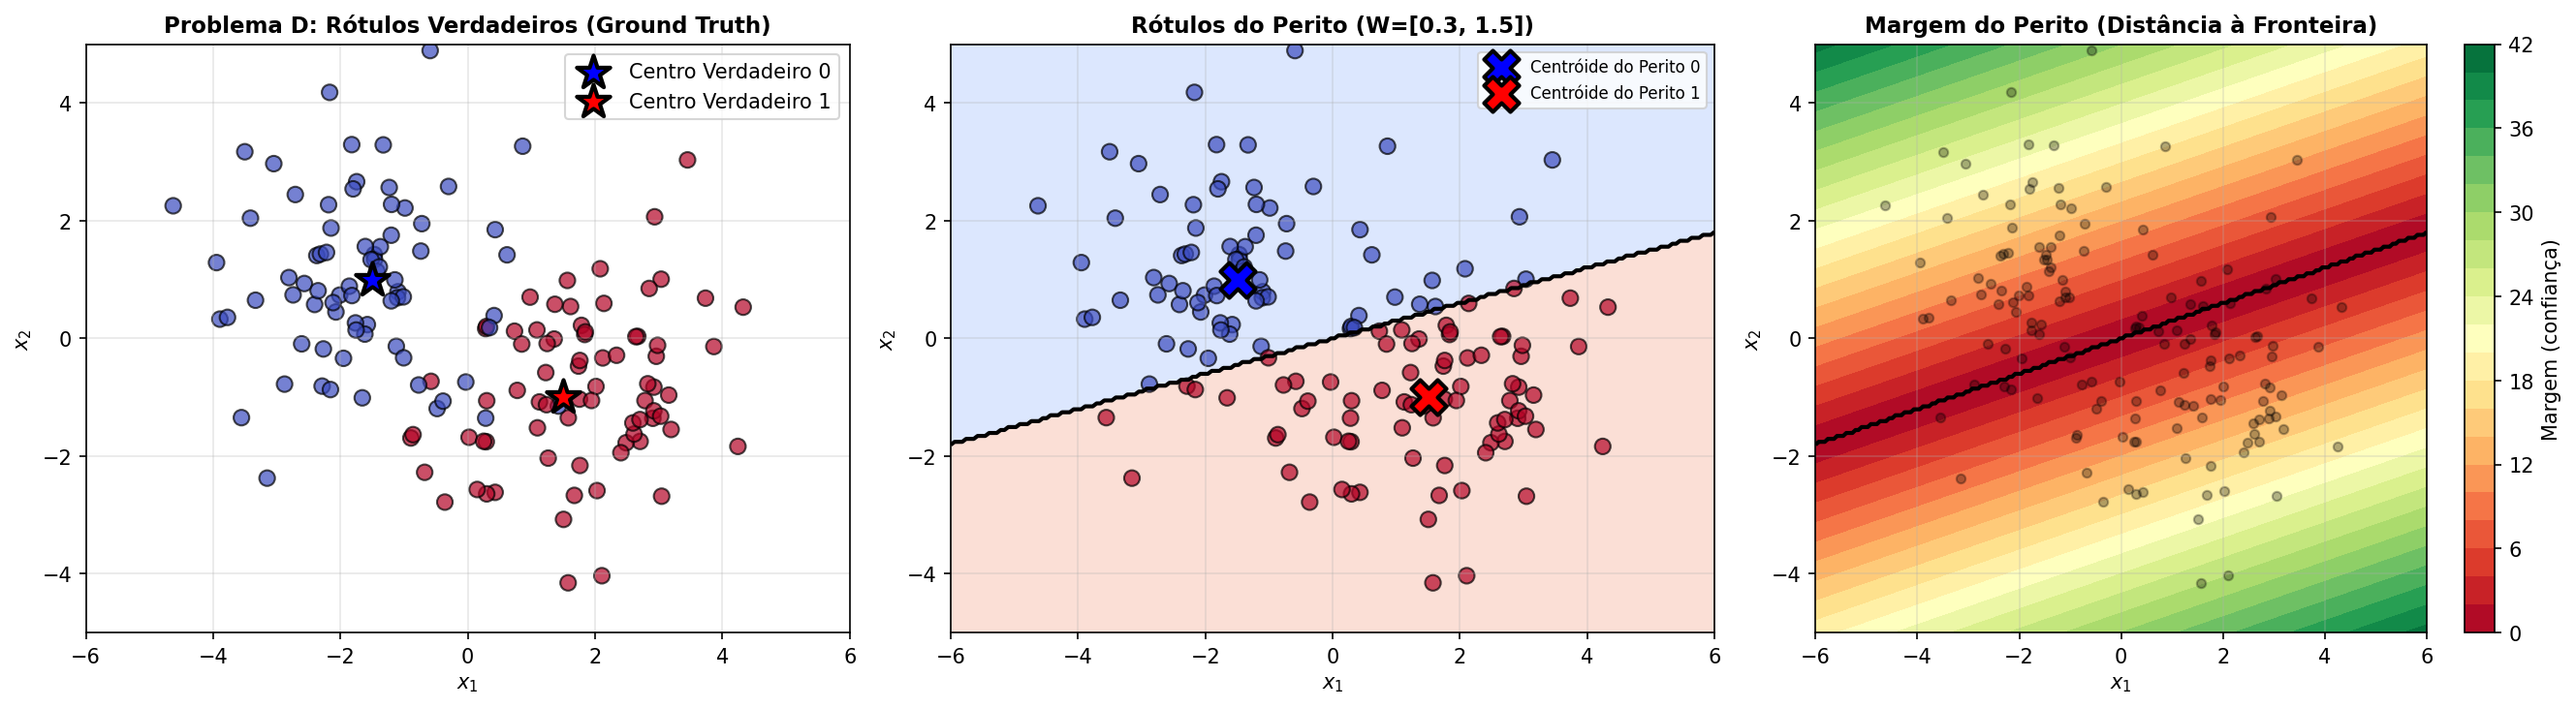
\includegraphics[width=\textwidth]{../06_problem_d_expert.png}
\end{center}
\end{columns}
\end{frame}

% ============================================================
% SLIDE 10: CONFIGURACOES
% ============================================================
\begin{frame}{Configurações de Execução --- Design de Variabilidade}
\small
\begin{block}{Objetivo}
Garantir que resultados não são artefato de uma configuração específica.
\end{block}

\begin{columns}
\column{0.5\textwidth}
\textbf{Parâmetros de robustez:}
\begin{itemize}
    \item Seeds: $\{42, 123, 7\}$ (3 sementes)
    \item Repetições: 3 por configuração
    \item Temperatura: $0.0$ (minimiza estocasticidade)
    \item Modelo: \texttt{gpt-4o-mini}
\end{itemize}

\column{0.5\textwidth}
\textbf{Variações de nomes de classes:}
\begin{itemize}
    \item \texttt{A/B} --- neutro
    \item \texttt{0/1} --- numérico
    \item \texttt{Positivo/Negativo} --- semântico
    \item \texttt{Azul/Vermelho} --- semântico
\end{itemize}
\vspace{0.2cm}
$\Rightarrow$ Detecta viés semântico do LLM
\end{columns}
\end{frame}

% ============================================================
% SLIDE 11: ALGORITMO 1 — PERCEPTRON
% ============================================================
\begin{frame}{Algoritmo 1 --- Perceptron Estruturado com Relaxação de Margem}
\small
\begin{block}{Ideia}
Busca iterativa dos pesos $W$ que maximizam a margem de separação.
\end{block}

\textbf{Procedimento:}
\begin{enumerate}
    \item \textbf{Busca binária} sobre $\gamma$ (margem mínima)
    \item Para cada $\gamma$, treina o perceptron até convergência ou limite de épocas
    \item \textbf{Atualização:} quando a métrica erra a classificação do LLM:
    \[
    w_i \leftarrow w_i + \eta \cdot \left[ (x_i - c_{\text{errado}})^2 - (x_i - c_{\text{correto}})^2 \right]
    \]
    \item Projeção: $w_i \leftarrow \max(w_i, 0)$ (não-negatividade)
    \item Retorna o $W$ com maior $\gamma$ que converge
\end{enumerate}
\end{frame}

% ============================================================
% SLIDE 12: ALGORITMO 2 — NNLS
% ============================================================
\begin{frame}{Algoritmo 2 --- Mínimos Quadrados (NNLS)}
\small
\begin{block}{Formulação}
\[
\min_{\mathbf{w} \geq 0} \| A\mathbf{w} - \mathbf{b} \|^2
\]
\end{block}

\textbf{Construção do sistema:}
\begin{itemize}
    \item Para cada ponto $\mathbf{x}$ classificado como classe $k$ pelo LLM:
    \[
    \sum_i w_i (x_i - c_{k,i})^2 \leq \sum_i w_i (x_i - c_{j,i})^2, \quad \forall j \neq k
    \]
    \item Reescrito como $A\mathbf{w} \leq \mathbf{b}$ e resolvido via NNLS (\texttt{scipy})
\end{itemize}

\textbf{Vantagens:}
\begin{itemize}
    \item Solução fechada (não iterativa)
    \item Garante $w_i \geq 0$ por construção
    \item Validação cruzada: se Perceptron e NNLS convergem para $W$ similar $\Rightarrow$ resultado robusto
\end{itemize}
\end{frame}

% ============================================================
% SLIDE 13: ALGORITMO 3 — LP
% ============================================================
\begin{frame}{Algoritmo 3 --- Programação Linear (Max-Margin)}
\small
\begin{block}{Formulação}
\[
\max_{\mathbf{w}, \gamma} \; \gamma \quad \text{s.a.} \quad
\sum_i w_i \left[(x_i - c_{j,i})^2 - (x_i - c_{k,i})^2\right] \geq \gamma, \; \forall (\mathbf{x}, k), j \neq k
\]
\[
\sum_i w_i = 1, \quad w_i \geq 0, \quad \gamma \geq 0
\]
\end{block}

\textbf{Características:}
\begin{itemize}
    \item Maximiza a margem mínima sobre todas as observações
    \item Solução via \texttt{scipy.optimize.linprog} (solver HiGHS)
    \item Normalização $\sum w_i = 1$ evita solução trivial
    \item Se $\gamma^* = 0$: separação perfeita impossível com métrica diagonal
\end{itemize}

\textbf{Interpretação:} $\gamma^* > 0$ indica que existe uma métrica diagonal que reproduz \textbf{todas} as decisões do LLM com margem positiva.
\end{frame}


% ============================================================
% PARTE 3 — FASE A: APRENDIZADO DA METRICA
% ============================================================

% ============================================================
% SLIDE 14: FASE A — DESCRICAO
% ============================================================
\begin{frame}{Fase A --- Aprendizado da Métrica (Zero-Shot)}
\begin{block}{Procedimento}
\begin{enumerate}
    \item LLM classifica \textbf{150 pontos} do Problema A em \textbf{zero-shot}
    \item Prompt contém apenas as coordenadas e pede classificação A ou B
    \item A partir das 150 decisões, aprende-se $\hat{W}_{\text{LLM}}$ via cada algoritmo
    \item $\hat{W}$ representa o \textbf{critério decisório implícito} do LLM
\end{enumerate}
\end{block}

\vspace{0.3cm}
\textbf{Nota:} $\hat{W}_{\text{LLM}}$ é \textbf{estimada/inferida}, não ``aprendida'' pelo LLM --- é o resultado da otimização inversa sobre as decisões observadas.
\end{frame}

% ============================================================
% SLIDE 15: FASE A — W APRENDIDO
% ============================================================
\begin{frame}{Fase A --- $\hat{W}$ Estimado e Fidelidade}
\small
\begin{columns}
\column{0.5\textwidth}
\textbf{$\hat{W}$ por algoritmo (seed=42, classes A/B):}

\begin{tabular}{lcc}
\toprule
\textbf{Algoritmo} & $\hat{w}_1$ & $\hat{w}_2$ \\
\midrule
Perceptron & 1.000 & 0.000 \\
NNLS & 0.202 & 0.798 \\
LP & 0.707 & 0.707 \\
\bottomrule
\end{tabular}

\vspace{0.3cm}
\textbf{Fidelidade} (métrica reproduz LLM):
\begin{itemize}
    \item Perceptron: \textbf{72.7\%}
    \item NNLS: \textbf{80.7\%}
    \item LP: \textbf{74.7\%}
\end{itemize}

\column{0.5\textwidth}
\begin{center}

\includegraphics[width=\textwidth]{../11_metric_errors_phase_a_seed42.png}
\end{center}
\end{columns}

\vspace{0.2cm}
\warn{Acurácia LLM vs.\ ground truth: apenas 30.7\%} --- mas a fidelidade mede se a métrica \textbf{reproduz o LLM}, não se o LLM acerta.
\end{frame}

% ============================================================
% SLIDE 16: FASE A — DISTRIBUICAO DE W
% ============================================================
\begin{frame}{Fase A --- Distribuição de $\hat{W}$ entre Seeds}
\begin{columns}
\column{0.5\textwidth}
\begin{itemize}
    \item $\hat{W}$ varia entre seeds
    \item Similaridade cosseno entre seeds: \textbf{0.53} (média)
    \item Seed 42: $\hat{W} = [1.0, 0.0]$ (Perceptron)
    \item Seeds 123, 7: $\hat{W} = [0.0, 1.0]$
    \item \warn{H5 em risco}: direção de $W$ instável
    \item CV da razão $w_1/w_2$: \textbf{258.9\%}
\end{itemize}
\column{0.5\textwidth}
\begin{center}

\includegraphics[width=\textwidth]{../10_w_distribution.png}
\end{center}
\end{columns}
\end{frame}

% ============================================================
% SLIDE 17: FASE A — COMPARACAO DE ALGORITMOS
% ============================================================
\begin{frame}{Fase A --- Comparação de Algoritmos}
\begin{columns}
\column{0.5\textwidth}
\small
\textbf{Concordância entre algoritmos:}
\begin{itemize}
    \item Cosseno Perc--NNLS: \textbf{0.73}
    \item Cosseno Perc--LP: \textbf{0.73}
    \item Cosseno NNLS--LP: \textbf{0.87}
\end{itemize}

\vspace{0.2cm}
\textbf{Fidelidade média (3 seeds):}
\begin{tabular}{lc}
\toprule
\textbf{Algoritmo} & \textbf{Fidelidade} \\
\midrule
Perceptron & 76.0\% \\
NNLS & 82.4\% \\
LP & 75.2\% \\
\bottomrule
\end{tabular}

\vspace{0.2cm}
NNLS e LP mais concordantes entre si; Perceptron mais divergente em seeds específicas.

\column{0.5\textwidth}
\begin{center}

\includegraphics[width=\textwidth]{../14_algorithm_comparison.png}
\end{center}
\end{columns}
\end{frame}


% ============================================================
% PARTE 4 — FASES B E C: CONSISTENCIA
% ============================================================

% ============================================================
% SLIDE 18: FASES B/C — DESCRICAO
% ============================================================
\begin{frame}{Fases B e C --- Teste de Consistência}
\begin{block}{Pergunta}
``A métrica aprendida na Fase A \textbf{generaliza} para problemas diferentes?''
\end{block}

\textbf{Procedimento:}
\begin{enumerate}
    \item Aplica $\hat{W}_{\text{LLM}}$ (Fase A) ao Problema B/C com centroides locais
    \item LLM classifica os mesmos pontos (zero-shot ou few-shot)
    \item Compara: classificação do LLM vs.\ predição da métrica
\end{enumerate}

\textbf{Métricas:}
\begin{itemize}
    \item \textbf{Consistência} (\%): fração de concordância LLM--métrica
    \item \textbf{Cohen's Kappa} ($\kappa$): concordância ajustada pelo acaso
    \item \textbf{F1-Score}: média harmônica de precisão e recall
\end{itemize}
\end{frame}

% ============================================================
% SLIDE 19: FASES B/C — RESULTADOS
% ============================================================
\begin{frame}{Fases B e C --- Resultados (Perceptron, classes A/B)}
\small
\begin{columns}
\column{0.5\textwidth}
\begin{tabular}{r|cc|cc}
\toprule
& \multicolumn{2}{c|}{\textbf{Prob.\ B}} & \multicolumn{2}{c}{\textbf{Prob.\ C}} \\
\textbf{n\_shot} & Cons. & $\kappa$ & Cons. & $\kappa$ \\
\midrule
0  & 64.0\% & 0.14 & 63.1\% & 0.14 \\
5  & 91.7\% & 0.82 & 92.7\% & 0.85 \\
10 & 96.3\% & 0.93 & 96.3\% & 0.93 \\
20 & 97.6\% & 0.95 & 93.3\% & 0.87 \\
40 & 97.6\% & 0.95 & 93.1\% & 0.86 \\
\bottomrule
\end{tabular}

\vspace{0.3cm}
\good{Salto dramático} de zero-shot para 5-shot: +27.7\% (B), +29.6\% (C)

\column{0.5\textwidth}
\begin{center}

\includegraphics[width=\textwidth]{../02_consistency_extended.png}
\end{center}
\end{columns}
\end{frame}

% ============================================================
% SLIDE 20: FASES B/C — DISCUSSAO
% ============================================================
\begin{frame}{Fases B e C --- Discussão}
\begin{block}{H1 --- Consistência}
\begin{itemize}
    \item Zero-shot: $\kappa \approx 0.14$ $\Rightarrow$ \warn{concordância fraca}
    \item Few-shot ($\geq 5$): $\kappa > 0.80$ $\Rightarrow$ \good{concordância substancial}
    \item \textbf{H1 parcialmente confirmada:} consistência \textbf{com} exemplos, não sem
\end{itemize}
\end{block}

\begin{block}{H2 --- Few-shot amplifica}
\begin{itemize}
    \item Exemplos rotulados pela métrica \textbf{aumentam drasticamente} a concordância
    \item 5 exemplos já bastam para $\kappa > 0.80$
    \item \good{H2 confirmada}
\end{itemize}
\end{block}

\textbf{Limitação:} fidelidade baixa na Fase A (72--81\%) $\Rightarrow$ base frágil para transferência em zero-shot.
\end{frame}

% ============================================================
% PARTE 5 — VIESES E SENSIBILIDADE
% ============================================================

% ============================================================
% SLIDE 21: VIES DE ORDEM DAS CLASSES
% ============================================================
\begin{frame}{Viés de Ordem das Classes}
\small
\begin{columns}
\column{0.5\textwidth}
\textbf{Pergunta:} Trocar ``A ou B'' por ``B ou A'' muda o resultado?

\vspace{0.2cm}
\begin{tabular}{l|cc}
\toprule
\textbf{Classes} & \textbf{B (\%)} & \textbf{C (\%)} \\
\midrule
A/B & 79.5 & 78.1 \\
B/A & 94.9 & 92.5 \\
\midrule
0/1 & 83.7 & 60.9 \\
1/0 & 76.7 & 82.8 \\
\midrule
Pos./Neg. & 75.3 & 70.5 \\
Neg./Pos. & 87.3 & 83.5 \\
\midrule
Azul/Verm. & 83.6 & 78.5 \\
Verm./Azul & 79.4 & 75.6 \\
\bottomrule
\end{tabular}

\column{0.5\textwidth}
\begin{center}

\includegraphics[width=\textwidth]{../15_class_order_bias.png}
\end{center}

\vspace{0.2cm}
\warn{Existe viés posicional}: inverter a ordem pode alterar consistência em até \textbf{+15.4\%} (B/A vs A/B).
\end{columns}
\end{frame}

% ============================================================
% SLIDE 22: NOMES DE FEATURES
% ============================================================
\begin{frame}{Nomes Semânticos de Features}
\begin{columns}
\column{0.5\textwidth}
\textbf{Pergunta:} Chamar as coordenadas de ``altura/peso'' muda $\hat{W}$?

\vspace{0.2cm}
\textbf{Variantes testadas:}
\begin{itemize}
    \item \texttt{x1/x2} --- neutro (padrão)
    \item \texttt{altura/peso} --- semântico
    \item \texttt{feature\_1/feature\_2} --- técnico
\end{itemize}

\vspace{0.3cm}
O LLM é \textbf{sensível} ao significado semântico das variáveis --- nomes como ``altura/peso'' podem ativar conhecimento prévio e alterar pesos implícitos.

\column{0.5\textwidth}
\begin{center}

\includegraphics[width=\textwidth]{../19_feature_names_effect.png}
\end{center}
\end{columns}
\end{frame}

% ============================================================
% SLIDE 23: VARIANTES DE PROMPT (1/2)
% ============================================================
\begin{frame}{Variantes de Prompt (1/2) --- Design}
\textbf{Pergunta:} Mudar o template do prompt muda a métrica $\hat{W}$ inferida?

\vspace{0.3cm}
\textbf{4 variantes testadas:}
\begin{description}
    \item[\texttt{default}] Template atual (baseline)
    \item[\texttt{geometric}] Adiciona contexto geométrico/espacial explícito
    \item[\texttt{chain-of-thought}] Pede raciocínio passo a passo antes da resposta
    \item[\texttt{tabular}] Apresenta coordenadas como tabela markdown
\end{description}

\vspace{0.3cm}
\textbf{Protocolo:}
\begin{itemize}
    \item Cada variante executa Fases A--C completas (zero-shot, classes A/B) em todas as seeds
    \item Compara $\hat{W}$ aprendido, consistência e $\kappa$
\end{itemize}
\end{frame}

% ============================================================
% SLIDE 24: VARIANTES DE PROMPT (2/2)
% ============================================================
\begin{frame}{Variantes de Prompt (2/2) --- Resultados}
\begin{columns}
\column{0.5\textwidth}
\begin{itemize}
    \item O scatter de $\hat{W}$ mostra se o prompt ``confunde'' a medição
    \item Se $\hat{W}$ muda entre variantes $\Rightarrow$ o prompt é um confundidor
    \item \warn{Implicação:} a métrica inferida pode não capturar algo intrínseco ao LLM, mas sim um artefato do prompt
\end{itemize}

\vspace{0.2cm}
\textbf{Resultado:} sensibilidade moderada --- variantes com contexto explícito tendem a alterar a distribuição de decisões.

\column{0.5\textwidth}
\begin{center}

\includegraphics[width=\textwidth]{../17_prompt_variant_comparison.png}
\end{center}
\end{columns}
\end{frame}


% ============================================================
% PARTE 6 — FASE D: LLM COMO APRENDIZ
% ============================================================

% ============================================================
% SLIDE 25: FASE D — DESCRICAO
% ============================================================
\begin{frame}{Fase D --- LLM como Aprendiz}
\begin{block}{Papel Invertido}
Agora o LLM \textbf{aprende} de um expert externo com métrica $W_{\text{expert}}$ conhecida.
\end{block}

\begin{enumerate}
    \item Expert gera rótulos no Problema D usando $W_{\text{expert}} = [0.3, 1.5]$
    \item LLM recebe exemplos few-shot rotulados pelo expert
    \item LLM classifica pontos novos
    \item \textbf{Pergunta:} ``O LLM consegue aprender o critério do expert?''
\end{enumerate}

\begin{center}
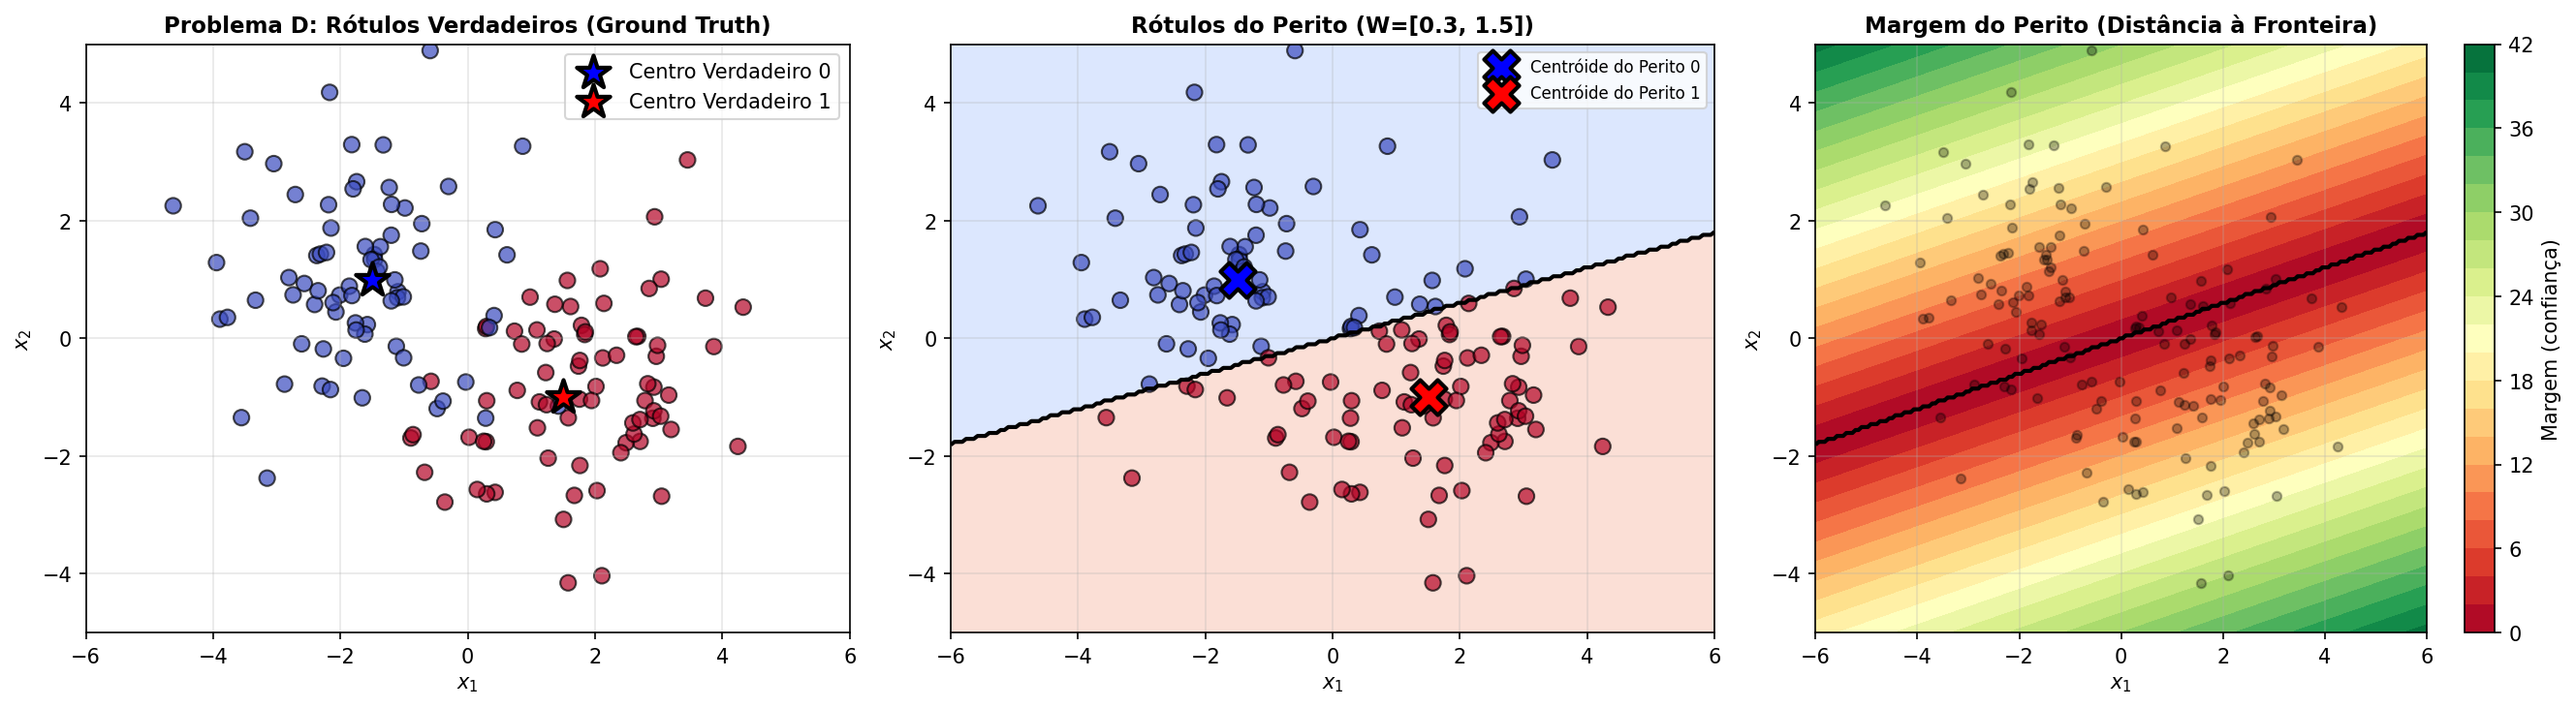
\includegraphics[width=0.35\textwidth]{../06_problem_d_expert.png}
\end{center}
\end{frame}

% ============================================================
% SLIDE 26: ESTRATEGIAS DE SELECAO
% ============================================================
\begin{frame}{Estratégias de Seleção de Exemplos}
\begin{columns}
\column{0.5\textwidth}
\textbf{4 estratégias:}
\begin{description}
    \item[\texttt{Easy}] Pontos longe da fronteira (alta margem)
    \item[\texttt{Hard}] Pontos próximos à fronteira (ambíguos)
    \item[\texttt{Mixed}] 50\% easy + 50\% hard
    \item[\texttt{Random}] Baseline sem estratégia
\end{description}

\vspace{0.2cm}
\textbf{Intuição H4:} exemplos hard deveriam ser mais informativos por definirem melhor a fronteira.

\column{0.5\textwidth}
\begin{center}
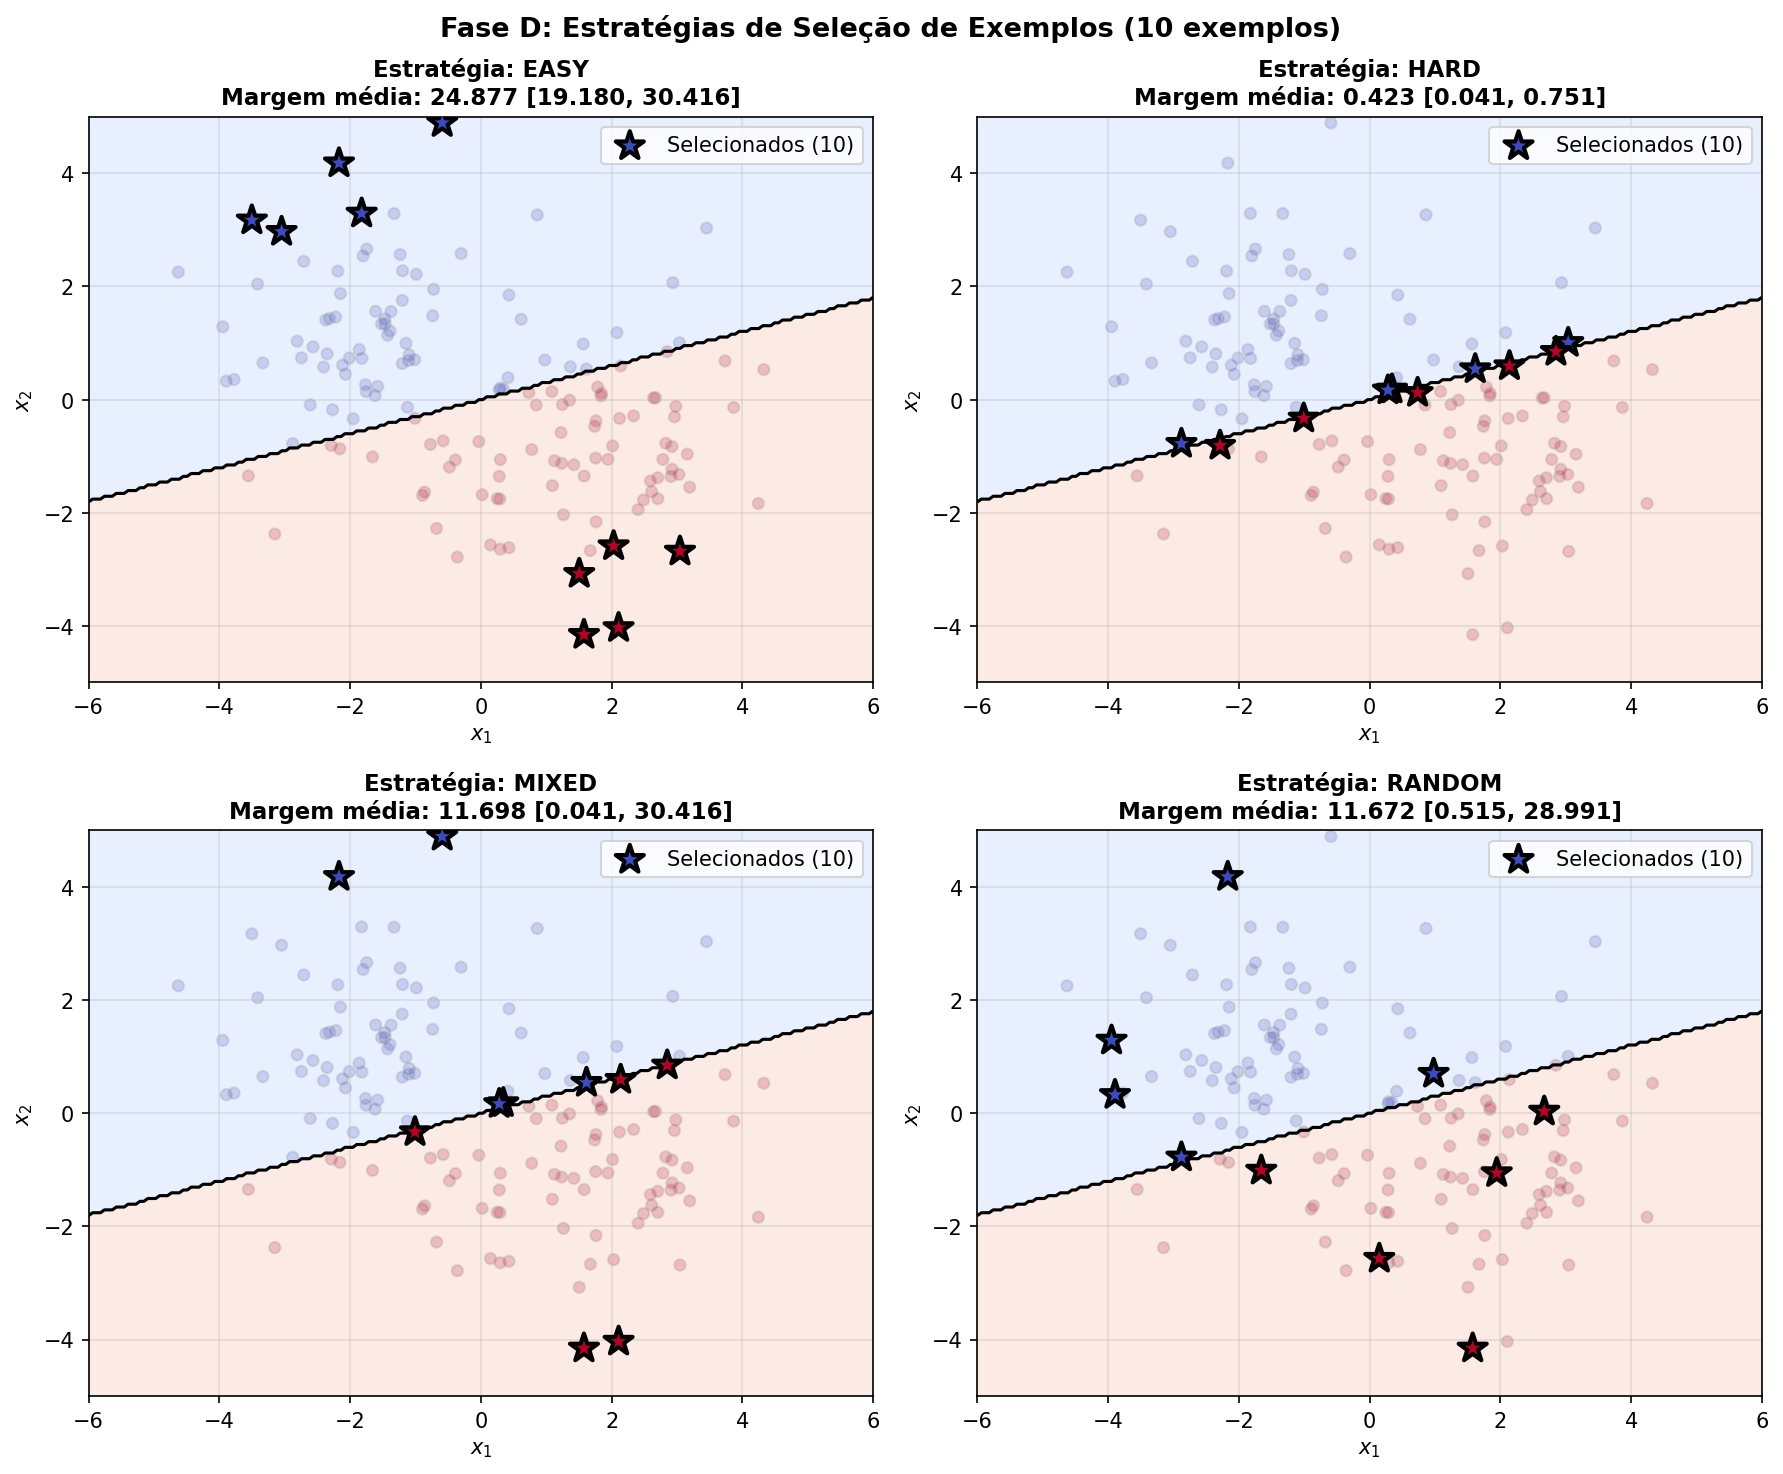
\includegraphics[width=\textwidth]{../07_phase_d_example_strategies.png}
\end{center}
\end{columns}
\end{frame}

% ============================================================
% SLIDE 27: FASE D — CURVAS DE APRENDIZADO
% ============================================================
\begin{frame}{Fase D --- Curvas de Aprendizado (Expert aniso\_x2)}
\small
\begin{columns}
\column{0.48\textwidth}
\begin{tabular}{r|cccc}
\toprule
\textbf{n} & \textbf{Easy} & \textbf{Hard} & \textbf{Mixed} & \textbf{Random} \\
\midrule
0  & 55.5 & 55.5 & 55.5 & 55.5 \\
5  & 78.6 & 52.5 & 83.7 & 84.4 \\
10 & 81.1 & 68.5 & 84.3 & 89.0 \\
20 & 83.6 & 84.5 & 89.5 & 93.2 \\
40 & 82.3 & 95.8 & 95.1 & 94.8 \\
\bottomrule
\end{tabular}

\vspace{0.2cm}
\good{H3 confirmada}: LLM melhora de 55.5\% (zero-shot) para até \textbf{95.8\%} (40-shot hard).

\column{0.52\textwidth}
\begin{center}

\includegraphics[width=\textwidth]{../08_phase_d_learning_curve.png}
\end{center}
\end{columns}
\end{frame}

% ============================================================
% SLIDE 28: FASE D — COMPARACAO DE ESTRATEGIAS
% ============================================================
\begin{frame}{Fase D --- Comparação de Estratégias}
\begin{columns}
\column{0.5\textwidth}
\small
\textbf{Acurácia média (todos n\_shot $>$ 0):}
\begin{enumerate}
    \item \good{Random: 90.4\%}
    \item Mixed: 88.1\%
    \item Easy: 81.4\%
    \item \warn{Hard: 75.3\%}
\end{enumerate}

\vspace{0.2cm}
\begin{block}{\warn{H4 REFUTADA}}
Exemplos easy (81.4\%) superam hard (75.3\%) consistentemente.
\end{block}

\textbf{Interpretação:} exemplos ``hard'' são \textbf{ambíguos} para o LLM. Exemplos fáceis funcionam como ``âncoras'' que definem regiões de cada classe.

\column{0.5\textwidth}
\begin{center}

\includegraphics[width=\textwidth]{../09_phase_d_strategy_comparison.png}
\end{center}
\end{columns}
\end{frame}

% ============================================================
% SLIDE 29: MULTIPLOS EXPERTS
% ============================================================
\begin{frame}{Múltiplos Experts}
\small
\textbf{3 configurações de expert testadas:}

\begin{center}
\begin{tabular}{llcl}
\toprule
\textbf{Expert} & $W_{\text{expert}}$ & Razão & \textbf{Descrição} \\
\midrule
\texttt{aniso\_x2} & $[0.3, 1.5]$ & $5.0\times$ & $x_2$ dominante (original) \\
\texttt{aniso\_x1} & $[1.5, 0.3]$ & $0.2\times$ & $x_1$ dominante (invertido) \\
\texttt{euclidean} & $[1.0, 1.0]$ & $1.0\times$ & Pesos iguais (Euclidiana) \\
\bottomrule
\end{tabular}
\end{center}

\vspace{0.2cm}
\textbf{Pergunta:} ``O LLM aprende igualmente bem critérios diferentes?''

\vspace{0.2cm}
\textbf{Validação oráculo} (oracle): todos os 3 algoritmos recuperam $W_{\text{expert}}$ com \textbf{fidelidade 100\%} no Problema D $\Rightarrow$ os algoritmos funcionam corretamente quando o classificador é consistente.

\vspace{0.2cm}
Similaridade cosseno (recuperado vs.\ real): \textbf{0.99--1.00} para Perceptron e LP.
\end{frame}

% ============================================================
% SLIDE 30: DILUICAO
% ============================================================
\begin{frame}{Experimento de Diluição}
\begin{columns}
\column{0.5\textwidth}
\textbf{Pergunta:} Adicionar exemplos fáceis ``dilui'' a informação dos difíceis?

\vspace{0.2cm}
\textbf{Design:} 4 hard fixos + easy progressivos:

\small
\begin{tabular}{cc|c}
\toprule
\textbf{Hard} & \textbf{Easy} & \textbf{Acc (\%)} \\
\midrule
4 & 0 & 56.8 \\
4 & 2 & 65.9 \\
4 & 4 & 81.7 \\
4 & 10 & 83.1 \\
4 & 16 & 86.9 \\
4 & 20 & 84.9 \\
\bottomrule
\end{tabular}
\normalsize

\vspace{0.2cm}
Fáceis \textbf{não diluem} --- performance melhora monotonicamente até 16 easy, com leve queda em 20.

\column{0.5\textwidth}
\begin{center}

\includegraphics[width=\textwidth]{../12_dilution_experiment.png}
\end{center}
\end{columns}
\end{frame}

% ============================================================
% SLIDE 31: VIES DE ORDEM DOS EXEMPLOS
% ============================================================
\begin{frame}{Viés de Ordem dos Exemplos Few-Shot (Recency Bias)}
\small
\begin{columns}
\column{0.5\textwidth}
\textbf{Pergunta:} A ordem dos exemplos few-shot afeta a performance?

\textbf{4 ordenações} (mesmos exemplos, estratégia mixed):
\begin{itemize}
    \item \texttt{class0\_first}: classe 0 primeiro
    \item \texttt{class1\_first}: classe 1 primeiro
    \item \texttt{shuffled}: ordem aleatória
    \item \texttt{alternating}: intercalado
\end{itemize}

\textbf{Resultados (seed=42, 10-shot):}
\begin{tabular}{l|c}
\toprule
\textbf{Ordem} & \textbf{Acc (\%)} \\
\midrule
class0\_first & 90.0 \\
class1\_first & 88.6 \\
shuffled & 90.0 \\
alternating & 88.6 \\
\bottomrule
\end{tabular}

\column{0.5\textwidth}
\begin{center}

\includegraphics[width=\textwidth]{../16_example_order_bias.png}
\end{center}
\end{columns}

\vspace{0.1cm}
\textbf{Conclusão:} efeito de recency bias \textbf{pequeno} ($\Delta \leq 1.4\%$).
\end{frame}


% ============================================================
% PARTE 7 — VALIDACOES ADICIONAIS
% ============================================================

% ============================================================
% SLIDE 32: VALIDACAO ORACLE
% ============================================================
\begin{frame}{Validação Oráculo (Sanity Check)}
\small
\begin{columns}
\column{0.5\textwidth}
\textbf{Objetivo:} verificar se os algoritmos \textbf{funcionam} quando o classificador é consistente.

\textbf{Protocolo:}
\begin{enumerate}
    \item Classificador sintético com $W$ conhecido gera rótulos
    \item Os 3 algoritmos tentam recuperar $W$
\end{enumerate}

\textbf{Resultados (Prob.\ D, aniso\_x2):}
\begin{tabular}{lcc}
\toprule
\textbf{Alg.} & \textbf{Cos.\ sim.} & \textbf{Fidelidade} \\
\midrule
Perceptron & 0.9999 & 100\% \\
NNLS & 0.9933 & 95.3\% \\
LP & 0.9999 & 100\% \\
\bottomrule
\end{tabular}

\column{0.5\textwidth}
\begin{center}

\includegraphics[width=\textwidth]{../22_oracle_w_recovery.png}
\end{center}
\end{columns}

\vspace{0.2cm}
\good{Se não recuperam $\Rightarrow$ problema é o algoritmo. Se recuperam $\Rightarrow$ problema é a inconsistência do LLM.}
\end{frame}

% ============================================================
% SLIDE 33: R3 — METODOLOGIA
% ============================================================
\begin{frame}{Projeção R3 --- Kernel Quadrático (Metodologia)}
\small
\textbf{Motivação:} testar se o LLM captura relações não-lineares entre features.

\textbf{Como funciona:}
\begin{itemize}
    \item Dados 2D originais $(x_1, x_2)$ $\Rightarrow$ adiciona $x_3 = x_1 \cdot x_2$
    \item Simula kernel quadrático sem sair do mundo linear
    \item LLM classifica 150 pontos com 3 coordenadas no prompt
    \item 3 algoritmos aprendem $W$ com 3 componentes
\end{itemize}

\textbf{Comparação:}
\begin{itemize}
    \item LLM com 2 features (R2) vs.\ LLM com 3 features (R3)
    \item Métrica aprendida em R3
\end{itemize}

\textbf{Pergunta:} o peso $w_3$ (associado a $x_1 \cdot x_2$) é relevante? O LLM ``percebe'' a interação?
\end{frame}

% ============================================================
% SLIDE 34: R3 — RESULTADOS
% ============================================================
\begin{frame}{Projeção R3 --- Resultados (seed=42)}
\small
\begin{columns}
\column{0.5\textwidth}
\textbf{$\hat{W}$ com 3 features:}
\begin{tabular}{lccc}
\toprule
\textbf{Alg.} & $w_1$ & $w_2$ & $w_3$ \\
\midrule
Perc. & 2.31 & 1.21 & 1.07 \\
NNLS & 0.05 & 0.28 & 0.03 \\
LP & 0.33 & 0.33 & 0.33 \\
\bottomrule
\end{tabular}

\vspace{0.2cm}
\textbf{Fidelidade R3:}
\begin{itemize}
    \item Perceptron: 86.0\%
    \item NNLS: 88.7\%
    \item LP: 90.0\%
\end{itemize}

\textbf{Concordância LLM(2feat) vs Métrica(3feat):} apenas \textbf{60.0\%} $\Rightarrow$ adicionar $x_3$ muda o comportamento do LLM.

\column{0.5\textwidth}
\begin{center}

\includegraphics[width=\textwidth]{../13_r3_vs_r2.png}
\end{center}
\end{columns}
\end{frame}

% ============================================================
% SLIDE 35: BASELINES — CONFIGURACAO
% ============================================================
\begin{frame}{Baselines Clássicos --- Configuração}
\small
\textbf{Pergunta:} ``O LLM faz algo que um classificador trivial não faria?''

\vspace{0.2cm}
\textbf{Mesmos exemplos} few-shot da Fase D $\rightarrow$ treino. \textbf{Mesmo} conjunto de teste.

\begin{center}
\begin{tabular}{lp{7cm}}
\toprule
\textbf{Classificador} & \textbf{Configuração} \\
\midrule
k-NN & $k = \min(n_{\text{shot}}, 5)$, ímpar. Distância euclidiana. \\
Logistic Regression & Regularização L2, \texttt{max\_iter=1000}. Fronteira linear. \\
SVM (RBF) & Kernel radial, $C=1.0$, $\gamma=$\texttt{scale}. Fronteira não-linear. \\
\bottomrule
\end{tabular}
\end{center}

\vspace{0.2cm}
\textbf{Avaliação:} mesmas métricas do LLM (acurácia vs.\ expert, $\kappa$, F1).
Testado para cada $(n_{\text{shot}}, \text{estratégia}, \text{expert}, \text{seed})$.
\end{frame}

% ============================================================
% SLIDE 36: BASELINES — RESULTADOS
% ============================================================
\begin{frame}{Baselines Clássicos --- Resultados}
\small
\begin{columns}
\column{0.5\textwidth}
\textbf{Acc vs.\ Expert (10-shot, easy, seed=42):}
\begin{tabular}{lc}
\toprule
\textbf{Classificador} & \textbf{Acc (\%)} \\
\midrule
k-NN (k=5) & 89.3 \\
Log.\ Regression & 89.3 \\
SVM (RBF) & 90.0 \\
\textbf{LLM} & \textbf{88.6} \\
\bottomrule
\end{tabular}

\vspace{0.2cm}
\textbf{Com exemplos hard (10-shot):}
\begin{tabular}{lc}
\toprule
k-NN & 62.1\% \\
\good{Log.\ Reg.} & \good{100.0\%} \\
SVM (RBF) & 48.6\% \\
LLM & 68.5\% \\
\bottomrule
\end{tabular}

\column{0.5\textwidth}
\begin{center}

\includegraphics[width=\textwidth]{../18_classical_baselines.png}
\end{center}
\end{columns}

\vspace{0.1cm}
\textbf{Conclusão:} LLM \textbf{não} é uniformemente superior. LR se destaca com exemplos hard (fronteira linear ideal). LLM tem vantagem em poucos exemplos ambíguos vs.\ k-NN/SVM.
\end{frame}


% ============================================================
% PARTE 8 — ANALISE ESTATISTICA
% ============================================================

% ============================================================
% SLIDE 37: ROBUSTEZ ENTRE SEEDS
% ============================================================
\begin{frame}{Robustez entre Seeds}
\begin{columns}
\column{0.5\textwidth}
\small
\textbf{Variabilidade dos resultados:}

\begin{itemize}
    \item Consistência B: \textbf{81.1\% $\pm$ 14.8\%}
    \item Consistência C: \textbf{77.9\% $\pm$ 16.8\%}
    \item $\hat{W}$ instável entre seeds (cosseno 0.53)
    \item Resultados few-shot mais estáveis que zero-shot
\end{itemize}

\vspace{0.2cm}
\textbf{Observação:} a alta variância em zero-shot reflete a \textbf{instabilidade intrínseca} do critério do LLM sem orientação externa.

\column{0.5\textwidth}
\begin{center}

\includegraphics[width=\textwidth]{../05_seed_comparison.png}
\end{center}
\end{columns}
\end{frame}

% ============================================================
% SLIDE 38: TESTES ESTATISTICOS
% ============================================================
\begin{frame}{Testes Estatísticos}
\small
\textbf{Bootstrap 95\% CI} (10.000 reamostras):

\begin{tabular}{llcc}
\toprule
\textbf{Métrica} & \textbf{n\_shot} & \textbf{Média} & \textbf{95\% CI} \\
\midrule
Consistência B (Perc) & 0 & 0.641 & [0.602, 0.675] \\
Consistência B (Perc) & 10 & 0.963 & [0.941, 0.985] \\
Consistência C (Perc) & 0 & 0.584 & [0.556, 0.609] \\
Consistência C (Perc) & 10 & 0.963 & [0.956, 0.970] \\
\bottomrule
\end{tabular}

\vspace{0.2cm}
\textbf{Teste pareado} (zero-shot vs.\ 10-shot):
\begin{itemize}
    \item Consistência B: $\Delta = +0.322$, CI95\% = $[+0.257, +0.360]$ \good{significativo}
    \item Consistência C: $\Delta = +0.373$, CI95\% = $[+0.342, +0.400]$ \good{significativo}
    \item Cohen's $d$: 7.08 (B), 19.81 (C) $\Rightarrow$ \good{efeito muito grande}
\end{itemize}

\textbf{Easy vs.\ Hard} (Fase D, 5-shot): $\Delta = +0.231$, CI95\% = $[+0.100, +0.340]$ \good{sig.}
\end{frame}


% ============================================================
% PARTE 9 — CONCLUSOES
% ============================================================

% ============================================================
% SLIDE 39: SINTESE — HIPOTESES
% ============================================================
\begin{frame}{Síntese dos Resultados --- Hipóteses}
\small
\begin{tabular}{c|l|c|l}
\toprule
& \textbf{Hipótese} & \textbf{Resultado} & \textbf{Evidência} \\
\midrule
\textbf{H1} & Consistência & \textcolor{orange}{\textbf{Parcial}} & $\kappa=0.14$ (zero) $\rightarrow$ 0.93 (10-shot) \\
\textbf{H2} & Few-shot amplifica & \good{Confirmada} & Salto de +30\% com 5 exemplos \\
\textbf{H3} & LLM como aprendiz & \good{Confirmada} & 55\% $\rightarrow$ 96\% (40-shot) \\
\textbf{H4} & Exemplos difíceis & \warn{Refutada} & Easy 81\% > Hard 75\% \\
\textbf{H5} & Estabilidade & \textcolor{orange}{\textbf{Parcial}} & $\hat{W}$ instável (cos=0.53) \\
\bottomrule
\end{tabular}

\vspace{0.3cm}
\textbf{Achados principais:}
\begin{itemize}
    \item LLMs \textbf{não} têm critério estável em zero-shot, mas \textbf{respondem muito bem} a exemplos
    \item Exemplos fáceis (``âncoras'') são mais eficazes que exemplos difíceis (``ambíguos'')
    \item A refutação de H4 é um \warn{achado relevante} sobre in-context learning
\end{itemize}
\end{frame}

% ============================================================
% SLIDE 40: CONTRIBUICOES
% ============================================================
\begin{frame}{Contribuições do Trabalho}
\begin{enumerate}
    \item \textbf{Framework de otimização inversa aplicado a LLMs}
    \begin{itemize}
        \item Abordagem nova: inferir critério decisório via Mahalanobis diagonal
        \item 3 algoritmos independentes validados com oráculo
    \end{itemize}

    \item \textbf{Evidência empírica sobre consistência decisória}
    \begin{itemize}
        \item LLMs são consistentes \textbf{com} orientação (few-shot), não sem
    \end{itemize}

    \item \textbf{Refutação de H4} --- achado valioso
    \begin{itemize}
        \item LLMs se beneficiam mais de exemplos prototípicos que fronteiriços
    \end{itemize}

    \item \textbf{Análise de sensibilidade abrangente}
    \begin{itemize}
        \item Viés de classe, features semânticas, prompt, ordem de exemplos
        \item Identificação de confundidores na medição
    \end{itemize}
\end{enumerate}
\end{frame}

% ============================================================
% SLIDE 41: LIMITACOES E TRABALHOS FUTUROS
% ============================================================
\begin{frame}{Limitações e Trabalhos Futuros}
\begin{columns}
\column{0.5\textwidth}
\textbf{Limitações:}
\begin{itemize}
    \item Apenas um modelo (\texttt{gpt-4o-mini})
    \item Dados sintéticos 2D apenas
    \item Métrica diagonal ($O(d)$ params)
    \item Temperatura fixa em 0.0
    \item LP infeasible em vários cenários
\end{itemize}

\column{0.5\textwidth}
\textbf{Trabalhos futuros:}
\begin{itemize}
    \item Múltiplos LLMs (Claude, Gemini, GPT-4o)
    \item Dados reais e alta dimensão (Iris, MNIST)
    \item Mahalanobis completa
    \item Fronteiras não-lineares (kernels, redes)
    \item Aplicações: auditoria de decisões de IA
    \item Variação de temperatura
\end{itemize}
\end{columns}
\end{frame}

% ============================================================
% SLIDE 42: AGRADECIMENTOS
% ============================================================
\begin{frame}{Agradecimentos}
\begin{center}
\vspace{1cm}
{\Large \textbf{Obrigado!}}

\vspace{1.5cm}
{\large Perguntas?}

\vspace{1.5cm}
\small
George Gomes\\
Programa de Pós-Graduação\\
2026
\end{center}
\end{frame}

\end{document}
